!en \section{Get me on, let me off}
!de \section{Mach' mich an, lass' mich aus}

!en At first the enhanced schema

!de Zuerst die erweiterte Schaltung

\begin{figure}[htbp]
  \centering
  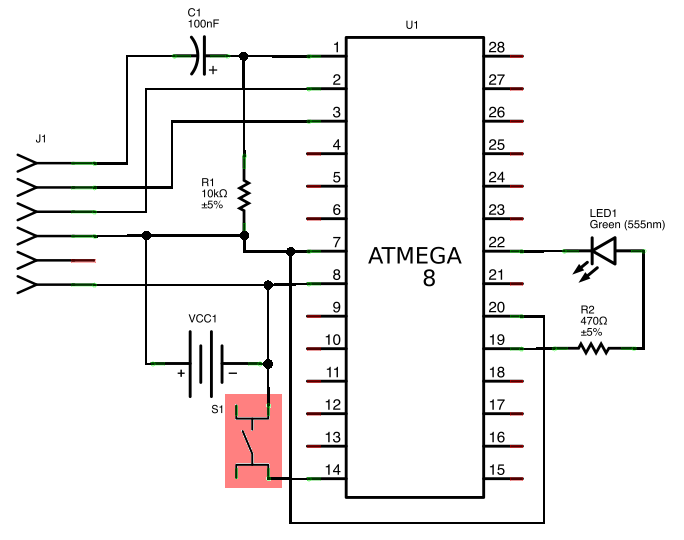
\includegraphics[width=120mm]{LED/S002_get-me-on-get-me-off_Circuit_schema.png}
!en   \caption{Get me on, get me off - Schema}
!de   \caption{Mach' mich an, lass' mich aus - Schaltplan}
  \label{atmega8-get-me-on-get-me-off-schema}
  \label{atmega8-get-me-on-get-me-off-schema}
\end{figure}


!en Second the code

!en Als zweites das Programm


\begin{lstlisting}
; LED/S002_get-me-on-get-me-off.asm

.DEVICE atmega8

.org 0x0000
            rjmp     start

start:
            sbi     DDRB,         5
            cbi     DDRB,         0
            sbi     PORTB,        0

main:
            sbic    PINB,         0
            rjmp    led_on
            cbi     PORTB,        5
            rjmp    led_ok
led_on:
            sbi     PORTB,        5
led_ok:
            rjmp    main
\end{lstlisting}

!en As you may have guessed, this code represents the 'second form of a standard program'. It does something before the loop - ones - but also does something in the main loop. This program is really busy as we will see in the next program.

!de We Du sicher schon vermutet hast ist dies bereits ein Programm der 'Zweiten Form'. Es tut nicht nur etwas vor der Endlosschleife, sondern ebenfalls etwas darin. Dieses Programm hat wirklich viel zu tun, wie im nächsten Programm noch sehen werden.



!en The first difference to the former program is, that we use an additional pin/bit. This time for input. To set this pin, bit 0 on port B at pin 14 of the micro controller, to input mode, we send a '0' to its data direction register (DDR). Further we send a '1' to this bit 0 of the port as if we would set the port to output +5V. But this bit is in 'output mode'. In this case, sending '1' to the bit at the port means: 'Switch on the internal pull-up resistor'.

!de Der erste Unterschied zum vorherigen Programm ist, dass wir ein zusätzliches Bein benutzen, diesmal um ein Eingangssignal zu erkennen. Um dieses Bein, Bit 0 an Port B = Bein 14 am MC, auf den Input Modus zu schalten, senden wir eine '0' an das entsprechende 'Data Direction Register' (DDR). Ausserdem senden wir eine '1' auf das Bit am entsprechenden Port. Was im Ausgabemodus bedeuten würde 'Schalet +5V an das Pin', heisst im Ausgabemodus: 'Schalten den pull-up Widerstand zu'.



!en After this, the signal read from this bit is 'ON' or '1'. To interact with the micro controller and change the signal to 'OFF', we need to pull-down the pin to GND.

:de Danach können wir vom Eingangsbein den Status 'EIN' oder '1' lesen. Um eine Reaktion am MC zu erreichen und das Eingangssignal auf 'AUS' oder '0' zu setzen, müssen wir das Beim auf Masse legen.



!en If we do so, our program switches the light off as long as we ground our input bit, which does not make real impressive application to boast around with. For us it is great anyway because we understand what happens!

!de Wenn wir das machen, schaltet unser Programm das Licht aus solange wir das Eingangsbein auf Masse legen. Das ist nicht direkt eine Anwendung mit der wir gross angeben können. Für uns ist es dennoch grossartig weil wir verstehen was passiert!



!en If you follow the programs flow:

\begin{enumerate}
!en   \item Initialise system and all connected devices
!de   \item Initialisiere das System und die angeschlossenen Geräte
!en   \item Read bit 0
!de   \item Lese Bit 0
!en   \item Set bit 5 accordingly
!de   \item Setze Bit 5 entsprechend
!en   \item Start with (2)
!de   \item Weiter bei (2)
\end{enumerate}

!en You may ask why we permanently output a signal that nearly never changes. Assuming our program reads the input bit one million times per second, a human will not be able to put any business to this program by flipping the switch on and off. If you pick on your signal line as fast as you can then in the eye of your program the signal nearly never changes.

!de Du wirst vielleicht fragen wollen, wieso ständig das gleiche Signal auf das Ausgabebit ausgegeben wird. Wenn wir einmal grob annehmen, dass unser Programm das Eingangsbit ca. eine Million mal pro Sekunde liest (eher 8 Mio. mal), ist einzusehen, dass ein Mensch mit einem Tasten kaum 'Last' für unseren MC erzeugen kann. Wenn Du auf dem Schalter einhämmerst so schnell Du kannst, passiert aus der Sicht des Micro Controllers so gut wir gar nichts, das Signal ändert sich dann für den MC in historischen Zeiträumen.


!en Is there room for optimisation? We believe not.

!de Kann man das optimieren? Wir glauben nicht.



!en Are there alternatives? Yes there are!

!de Gibt es andere Lösungen? Ja, die gibt es!



!en We could save the output status, compare the status from the input bit with the stored status the light was set to and only change the output signal if the input signal has changed.

!de Wir könnten den zuletzt ausgegebenen Status speichern. Dann könnten wir in der nächsten Programmschleife prüfen ob sich der eingelesene Status zum vorherigen Status geändert hat und nur dann ein Signal an das Bein ausgeben, wenn eine solche Änderung vorliegt.



!en This sounds easy, but it is not! It is not only not easy, it is dangerous, costly and complicated. And it is of no use, because you do a lot of commands without any effect.

!de Das klingt einfach, ist es aber leider nicht! Es ist nicht nur nicht einfach, es ist gefährlich, kostspielig und kompliziert. Und es ist effektiv sinnlos weil wir eine Menge Aufwand treiben würden, ohne dass sich etwas verbessert.



!en The concept is dangerous because you may be out of synchronisation with your light. In this case you light may react inverse to your intension or does not react at all.

!de Das Konzept ist gefährlich weil das Programm aus dem Rhythmus kommen könnte. Danach würde es falsch herum arbeiten oder überhaupt nicht mehr auf Eingangssignale reagieren.



!en It is costly not only because the program would be much larger but you need to eat up one CPU register (for storing the status) and we only have 32 of them at all.

!de Es ist kostspielig weil das Programm nicht nur viel grösser würde, wir würden ausserdem ein CPU Register verbrauchen (um den Status zu speichern) und wir haben total nur 32 Stück!



!en And it is complicated because you have to synchronise two entities (the light and the status register) to generate one effect. Which is a major risk and drawback.

!de Und es ist kompliziert weil wir zwei unabhängige Einheiten zusammenhalten müssen (das Licht und das Statusregister) um nur einen Effekt zu erzielen. Das ist ein grosses Risiko und ein Nachteil gegenüber der vorliegenden Lösung.



!en Because of this, we might be right in our assumption that the developers of our \at micro controller created the chip in such a way that nothing happens if we switch on a bit that is ON already.

!de Deswegen liegen wir vielleicht nicht falsch mit der Vermutung, dass die Entwickler unseres \at Micro Controllers ihren Chip so entwickelt haben, dass in Wirklichkeit gar nichts gemacht wird, wenn wir eine '1' auf ein Steuerbit senden, dass bereit auf '1' gesetzt ist.



!en Another alternative may be to 'stop' the program as long as it waits for the input signal to change. This may be possible, but it lies far behind our current knowledge.

!de Ein anderer Vorloche könnte sein, das Programm anzuhalten solange wir auf ein Eingangssignal warten. Das sollte möglich sein, liegt aber momentan weiter über unseren Kenntnissen.



!en There is no command that makes the micro controller wait for an input signal. But there are ways to reach a similar effect.

!de Es gibt keinen Befehl, der einen MC veranlasst, auf ein Eingangssignal zu warten. Aber es ist durchaus möglich, ein Programm zu entwickeln, dass so wirkt als gäbe es einen solchen.



!en Which means, for now we are out of options and have to stay with the solution as presented in this section. But we will come to status management later.

!de das heisst, momentan haben wir keine Wahl und müssen bei der vorliegenden Lösung bleiben. Aber bald werden wir auch ins Reich der Statusverwaltung vordringen.
